\documentclass [handout]{beamer}
\usetheme{metropolis}
%\mode<presentation>
%\mode<handouts>

\AtBeginSection[]{
  \begin{frame}
  \vfill
  \centering
    \begin{beamercolorbox}[sep=8pt,center,shadow=true,rounded=true]{title}
    \usebeamerfont{title}\insertsectionhead\par%
    \end{beamercolorbox}
  \vfill
  \end{frame}
}

\title[Discrete Math]{A Short Course in Discrtete Mathematics for the Computer Science Undergraduate}
\author{Dale Fletter}
\institute{UC Davis, ECS20, Summer Session 2}
\date{}
\usepackage{graphicx} % support the \includegraphics command and options
\usepackage {graphics}
\graphicspath{ {../../Outline-tex/illustrations/} }






\begin{document}
\begin{frame}
\titlepage
\end{frame}

\section{Sets}
\begin{frame}{Definition of Set}
A set is an unordered collection of objects. The objects are called elements or members. The set contains its members and we say the members are elements of the set. We generally name sets using capital letters and variables in the set using lowercase. We use the notation $a \in A$ to designation that the object refered to as $a$ is an element of the set $A$.
\end{frame}

\begin{frame}
Can the SAME object be in a set twice???

NO.

The set of \{4,6,2\} is the same collection as \{2,4,6\} and \{2,2,4,4,6,6\}.
\end{frame}



\begin{frame}{Describing Set Membership}
We can describe the members of the set in different ways. We can \textbf{enumerate} them or we can describe some property that all members possess. For instance the set of English vowels can be listed like this with the elements between braces and separated by commas: $V = \{a,e,i,o,u\}$. But I can also just say $V= \{the English vowels\}$ and both define the same set. 
\end{frame}

\begin{frame}
Set enumeration often uses the convention of starting a pattern and leaving it to the reader to fill in. This uses the ellipsis (\ldots) to designate that as in this example:
\begin{displaymath}
\{10,20,30, \ldots \}
\end{displaymath}
which defines the set of all multiples of 10.
\end{frame}

\begin{frame}{Set Builder Notation}
We can use predicate logic to define sets. A predicate takes on the value of true when a property is present in an object. So if we define a predicate T that is true when an integer is divisible by three, we can define a set of integers that satisfy this predicate. We write that like this:
\begin{displaymath}
\{x | T(x) \} 
\end{displaymath}
which we read as `The set of all x such that T(x)' which means where T(x) is true. 
\end{frame}

\begin{frame}
In the last slide there was an implied domain of discourse which was the set of integers. We have many sets used in mathematics with symbols as shorthand for those sets.
\end{frame}

\begin{frame}
\begin{align*}
\mathbb{N}&=\{1,2,3, \dots \} \text {the set of \textbf{natural numbers} }  \\
 \mathbb{Z}&=\{\dots -3,-2,-1,0,1,2,3, \dots\}  \text{The set of } \textbf{integers} \\
 \mathbb{Q}&=\{\dfrac{p}{q} | p \in \mathbb{Z}, q \in \mathbb{Z}, q \neq 0 \} \text{The set of \textbf{rational numbers}} \\
 \mathbb{R}&=\{ \text{the set of }\textbf{real numbers}   \}  \\
 \mathbb{C}&=\{ \text{the set of }\textbf{complex numbers} \}  \\
 \mathbb{B}&=\{0,1\} \text{ the set of \textbf{a set of binary symbols} }  \\
 \end{align*}
 \end{frame}
 
 \begin{frame}
 It is common to decorate the common set symbols with a superscript + or - to indicate the positive subset: \\
$\mathbb{Z}^+ is the set of positive integers$ for example.
 \end{frame}
 
 
 \begin{frame}
 When using set builder notation we can defined the domain of discourse by restricting the set of objects:
\begin{displaymath}
 D=\{x\in \mathbb{Z}^+ | x \text{ is odd }, x<100\}
 \end{displaymath}
 \end{frame}
 
 \begin{frame}
 Sets are often protrayed as Venn Diagrams \ldots
 \begin{figure}[htbp]
   \centering
   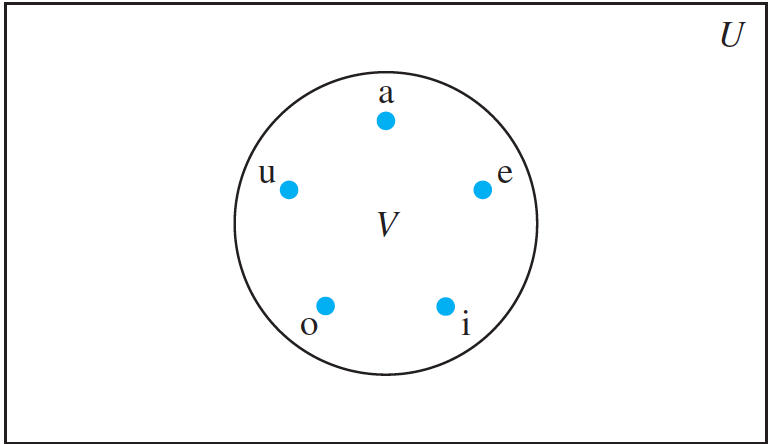
\includegraphics [width=2in]{Figure-2-1-1-VennDiagramOfVowels}
   \caption{VennDiagramOfVowels}
   \label{figure:VennDiagramOfVowels}
   \end{figure}
 \end{frame}
 
 \begin{frame}
 A Vennn diagram has a large rectangle called $U$ that represents the domain of discourse. This domain is called the universe or the \textbf{universal set} and designated as $U$. When specific elements of a set are to be discussed they are labeled dots in the diagram. The circle(s) represent the sets being discussed.
 \end{frame}
 
 \begin{frame}
 Sometimes the set contains no elements. Consider \{odd numbers divisible by 2\}. Such a set is called the null set or empty set and is designated as $\emptyset$ or by a pair of braces with nothing between. Be careful to never confuse $\emptyset$ with $\{\emptyset\}$.
 \end{frame}
 
 \begin{frame}{Set Cardinality}
 Let $S$ be a set. If there are exactly $n$ distinct elements in $S$ where $n$ is a nonnegative integer, we say that $S$ is a \textit{finite set} and that $n$ is the \textit{cardinality} of $S$. The cardinality of $S$ is denoted by $|S|$. Otherwise $S$ is an \textit{infinite} set. The cardinality of the empty set is 0.
 \end{frame}
 
 \begin{frame}{Programming Language Datatypes are Finite Sets}
 Note that many mathematical sets are infinite unlike the datatypes that are used to represent them in a computer. 
 \end{frame}
 
 \begin{frame}{Set Equality}
 Two sets are called \textit{equal} if, and only if, they have the same elements. That is, if $A$ and $B$ are sets, then $A$ and $B$ are equal if 
 \begin{displaymath}
 \forall x(x\in A \leftrightarrow x\in B).
 \end{displaymath}
 We write $A=B$ if $A$ and $B$ are equal sets.
 \end{frame}
 
 \begin{frame}{Subsets}
 The set $A$ is said to be a \textit{subset} of $B$ if and only if every element of $A$ is also an element of $B$. We use the notation $A\subseteq B$ to indicate that $A$ is a subset of $B$. If $A$ is a subset of $B$, this statement is true:
\begin{displaymath}
 \forall x(x\in A \rightarrow x\in B)
 \end{displaymath}
 \end{frame}
 
 \begin{frame}
 Every nonempty set has two subsets, itself and the emptyset. 
Proof. Let $S$ be a nonempty set. To show that $\emptyset \subseteq S$, we must show that $\forall x(x\in\emptyset \rightarrow x \in S)$ is true. The emptyset contains no elements so the antecedent of the conditional statement is always false and therefore the conditional statement is always true. Since the conditional statement is always true, the emptyset meets the definition for a subset of $S$. Proving that a set is a subset of itself is easily proved and left as a challenge.
 
 This is an example of a \textit{vacuous proof}. There are many definitions that will include edge cases when the antecedent of the conditional statement can never be true.
 \end{frame}
 
 \begin{frame}
 Sometimes it is helpful to talk about subsets that may not be equal to another set. We call these \textit{proper subsets} and can be denoted with $\subset$. Set $A$ is a proper subset of $B$ if
 \begin{displaymath}
 \forall x(x\in A \rightarrow x\in B) \land \exists x(x \in B \land x \not \in A)
 \end{displaymath}
 \begin{figure}[htbp]
   \centering
   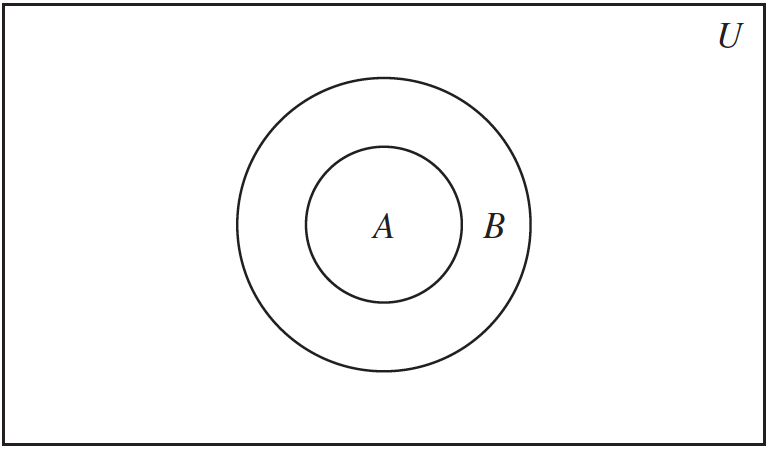
\includegraphics [width=2in]{Figure-2-1-2-VennDiagramOfAsubsetB}
   \caption{Venn Diagram Showing A as a Proper Subset of B}
   \label{figure:VennDiagramOfSubset}
   \end{figure}
 \end{frame}
 
 \begin{frame}{Powersets}
 Sets can contain other objects and sets are objects. So sets can contain other sets. One such set of sets is that set which contains all the possible subsets of another set. We know the empty set only contains itself while the set which contains a single element has two subsets. You can see that a set of two objects has four subsets. 

We define the set of all subsets of a given set as the \textit{powerset}. We designate the powerset of all subsets possible on a set $A$ as $\mathcal{P}(A)$. Remember that the powerset is a set of sets. Each member of the powerset is a set.
 \end{frame}
 
 \begin{frame}
 Example: What is $\mathcal{P}(\emptyset)$? \\
 This set has no elements. 
 $\{\emptyset\}$ \\
 What is the $\mathcal{P}(\{\emptyset\})$? \\
 This set has one element.
 $\{\emptyset, \{\emptyset\} \}$
 \end{frame}
 
 \begin{frame}{Ordered Tuples}
 While sets are unordered we often need an ordered collection. For example we have ordered pairs and we know that the ordered pair $(3,4)$ is different from the ordered pair $(4,3)$. We now define an ordered n-tuple. The \textit{ordered n-tuple} $(a_1,a_2,\ldots ,a_n)$ is the ordered collection that has $a_1$ as its first element, $a_2$ as its second element, \ldots, and $a_n$ as its $n$th element. We say that two ordered $n$-tuples are equalif and only if each corresponding pair of their elements is equal. The tuples $(a_1,a_2,\ldots,a_n)= (b_1,b_2, \ldots,b_n)$ only if $a_i=b_i$ for $i=1,2,\ldots ,n$.
 \end{frame}
 
 \begin{frame}{Cartesian Product of Two Sets}
 Let $A$ and $B$ be sets. The\textit{Cartesian product} of $A$ and $B$, denoted $A \times B$, is the set of all ordered pairs $(a,b)$, where $a\in A$ and $b \in B$. Hence, 
 \begin{displaymath}
 A \times B = \{(a,b) | a\in A \land b\in B\}
 \end{displaymath}
 \end{frame}
 
 \begin{frame}{Cartesian Product}
 The \textit{Cartesian product} of the sets $A_1,A_2, \ldots ,A_n$, denoted by $A_1 \times A_2 \times \ldots A_n$, is the set of ordered $n$-tuples $(a_1,a_2,\ldots,a_n)$, where $a_i\in 1,2,\ldots,n$.
 
 We use the notation $A^2$ to denote $A\times A$, the Cartesian product of the set $A$ with itself. In general
 \begin{displaymath}
 A^n=\{(a_1,a_2,\ldots,a_n) | a_i\in A \text{ for } i=1,2, \ldots ,n\}
 \end{displaymath}
 \end{frame}
 
 \begin{frame}{Truth Sets}
  Given a predicate $P$, and a domain $D$, we define the \textbf{truth set} of $P$ to be the set of elements $x$ in $D$ for which $P(x)$ is true. The truth set of $P(x)$ is denoted by $\{x\in D | P(x)\}$.
 \end{frame}
 
 \begin{frame}{Set Union}
 Let $A$ and $B$ be sets. The \textit{union} of the sets $A$ and $B$, denoted by $A \cup B$, is the set that contains those elements that are either in $A$ or in $B$, or in both.

$A \cup B = \{x |x\in A \lor x \in B\}$
 \end{frame}
 
 \begin{frame}{Set Intersection}
 Let $A$ and $B$ be sets. The \textit{intersection} ofthe sets $A$ and $B$, denoted by $A\cap B$, is the set containing those elements in both $A$ and $B$.
 
 $A\cap B=\{x|x\in A \land x\in B\}$
 \end{frame}
 
 \begin{frame}{Disjoint Sets}
 Two sets are called \textit{disjoint} if their intersection is the empty set.
 \end{frame}
 
 \begin{frame}{Set Difference}
 Let $A$ and $B$ be sets. The \textit{difference} of $A$ and $B$, denoted by $A-B$ or sometimes by $A \backslash B$, is the set containing those elements that are in $A$ but not in $B$ is also called the \textit{complement of B with respect to A}.
 \end{frame}
 
 \begin{frame}{Set Complement}
 Let $U$ be the universal set. The \textit{complement} of the set $A$, denoted by $\overline{A}$, the complement of $A$ with respect to $U$. Therefore, the complement of the set $A$ is $U-A$.
 \begin{displaymath}
 \overline{A}=\{x\in U | x\in A\}.
 \end{displaymath}
 \end{frame}
 
 \begin{frame}{Set Identities}
 
 
 \end{frame}
 
 \begin{frame}{Membership Table}
 
 \end{frame}
 
 \begin{frame}{Generalized Unions and Intersections}
 \end{frame}
 
 \begin{frame}{Multisets or Bags}
 \end{frame} 
 

\end{document}